\documentclass[sigconf]{acmart}

%% Using the option "anonymous" will produce "Anonymous Author(s)"
%% for double-anonymized review. Upon acceptance, remove this option
%% and set the authors' names and affiliations using the corresponding
%% commands.

%% CBSoft uses an ACM-like format without the ACM Reference block.
%% The following warning from acmart can be safely ignored:
%% "ACM reference format is mandatory for papers over one page."
\settopmatter{printacmref=false}
\renewcommand\footnotetextcopyrightpermission[1]{} % removes footnote with conference information in first column

%% CBSoft uses an ACM-like format without a copyright note.
\setcopyright{none}

%% These commands are for a PROCEEDINGS abstract or paper.
\acmConference[SBES 2026]{40th Brazilian Symposium on Software Engineering}{September 8–11, 2026}{São Paulo, SP, Brazil}

% CBSoft uses an ACM-like format without CCS Concepts.
% The following warning from acmart can be safely ignored:
% "CCS concepts are mandatory for papers over two pages."

%% \BibTeX command to typeset BibTeX logo in the docs
\AtBeginDocument{
    \providecommand\BibTeX{{Bib\TeX}}
}

%% Only for papers written in PORTUGUESE: 
%% comment out the following three lines
%\renewcommand\abstractname{Resumo}
%\renewcommand\keywordsname{Palavras-chave}
%\renewcommand\refname{Referências}

%% end of the preamble, start of the body of the document source.

% ------------------------------------------------------------
% Authors: please make sure to read the checklist comments
% provided at the end of this document before submission.
% ------------------------------------------------------------
\begin{document}

%% The "title" command has an optional parameter,
%% allowing the author to define a "short title" to be used on the page 
%% headers.
\title{The Name of the Title Is Hope}

%% The "author" command and its associated commands are used to define
%% the authors and their affiliations.
%% Of note is the shared affiliation of the first two authors, and the
%% "authornote" and "authornotemark" commands
%% used to denote shared contribution to the research.
\author{FirstName Surname1stAutor}
\affiliation{
  \institution{DepartmentName, Institution/UniversityName}
  \city{City}
  \country{Country}
}
\email{email@email.com}

\author{FirstName Surname}
\affiliation{
  \institution{DepartmentName, Institution/UniversityName}
  \city{City}
  \country{Country}
}
\email{email@email.com}

\author{FirstName Surname}
\affiliation{
  \institution{DepartmentName, Institution/UniversityName}
  \city{City}
  \country{Country}
}
\email{email@email.com}

\author{FirstName Surname}
\affiliation{
  \institution{DepartmentName, Institution/UniversityName}
  \city{City}
  \country{Country}
}
\email{email@email.com}

\author{FirstName Surname}
\affiliation{
  \institution{DepartmentName, Institution/UniversityName}
  \city{City}
  \country{Country}
}
\email{email@email.com}

\author{FirstName Surname}
\affiliation{
  \institution{DepartmentName, Institution/UniversityName}
  \city{City}
  \country{Country}
}
\email{email@email.com}

\author{FirstName Surname}
\affiliation{
  \institution{DepartmentName, Institution/UniversityName}
  \city{City}
  \country{Country}
}
\email{email@email.com}

\author{FirstName Surname}
\affiliation{
  \institution{DepartmentName, Institution/UniversityName}
  \city{City}
  \country{Country}
}
\email{email@email.com}

\author{FirstName Surname}
\affiliation{
  \institution{DepartmentName, Institution/UniversityName}
  \city{City}
  \country{Country}
}
\email{email@email.com}

%% By default, the full list of authors will be used on the page
%% headers. This list is often too long and will overlap
%% other information printed in the page headers. 
%% This command allows the author to define a more concise list
%% of authors' names for this purpose.
\renewcommand{\shortauthors}{Surname1stAuthor et al.}
\renewcommand{\shorttitle}{The Name of the Title Is Hope}

%% The abstract is a short summary of the work the paper presents.
\begin{abstract}
This ACM-like template, derived from the original \texttt{acmart} document class, is intended to support the preparation of scientific papers for the symposia and workshops that compose CBSoft. It preserves the visual identity and structural organization of the ACM consolidated format while adapting its elements to comply with the editorial and formatting guidelines adopted by the Brazilian Computer Society. This template can be used for both review and camera-ready versions, allowing authors to prepare their manuscripts with minimal structural changes. The abstract text must be written as a single continuous paragraph, without paragraph breaks.
\end{abstract}

%% Keywords. The author(s) should pick words that accurately describe
%% the presented work. Separate the keywords with commas.
\keywords{Do, Not, Use, This, Code, Put, the, Correct, Terms, for, Your, Paper}

%% This command processes the author, affiliation, and title
%% information and builds the first part of the formatted document.
%% "frenchspacing" avoids an additional space after a period at the end of a sentence.
\frenchspacing
\maketitle

\section{Introdução}

Diante dos recentes avanços de modelos de IA (inteligência artifical), a Engenharia de Software vem se modificando para se adequar tais práticas. As ferramentas baseadas em IA tem auxiliado a apoiar a sociedade em tarefas cotidianas e do trabalho, dentro do ciclo de desenvolvimento, podemos apontar uma ajuda na licitação de requisitos, geração de código, testes e documentação.

De forma mais recente, agentes autônomos de programação tem se demonstrado capaz de implementar funcionalidades completas a partir de uma descrição usando linguagem natural, reduzindo assim o esforço manual necessário dos desenvolvedores de software.

Apesar dos avanços tecnológicos e da chegada de novos modelos poderosos, ainda é possível observar que a qualidade dos artefatos produzidos por agentes depende diretamente da qualidade das instruções fornecidas para eles. Requisitos incompletos, ambíguos e com uma estrutura errada podem gerar resultados inconsistentes durante o processo de desenvolvimento, aumentando o retrabalho e o número de interações necessárias para concluir tal tarefa. Por conta disso, é necessário utilizar técnicas avançadas de Engenharia de Prompt e refinamento de requisitos, para melhorar a comunicação entre desenvolvedores humanos e agentes baseados em Large Language Models (LLM).

Paralelo a isso, observa-se o surgimento de diversas abordagens diferentes para conseguirmos utilizar tais LLMs, dentre elas a utilização de múltiplos agentes, na qual cada um assume responsábilidade específica dentro do processo de desenvolvimento. Nesse cenário, um agente pode atuar com o refinamento dos requisitos enquanto outro é responsável pela implementação do código, reproduzindo de forma simplificada os papéis tradicionais que vemos nos profissionais do mercado de trabalho.

Este trabalho irá investigar uma abordagem de desenvolvimento orientada por agentes baseados na separação das atividades de refinamento de requisito e implementação de software. Como base para o estudo, foi desenvolvido um software para auxiliar a produção de textos acadêmicos utilizando \LaTeX{}, cujas funcionalidades e elementos de interface foram concebidos por meio de um processo de desenvolvimento assistido por agentes. A proposta consiste em utilizar um agente especializado em transformar as descrições e requisitos de funcionalidades escritas por humanos em prompts robustos que posteriormente serão utilizados como entrada para um agente autônomo de programação responsável por tal implementação de solução.

Como objetivo do trabalho, busca-se analisar o potencial dessa estratégia para apoiar o desenvolvimento de software assistido por IA. Serão discutidos seus benefícios, limitações e implicações para a Engenharia de Software. Para isso, foi conduzido um estudo de caso no qual os requisitos da aplicação forma inicialmente definidos por um desenvolvedor humano, refinados por um agente especializado e posteriormente implementados por um agente autônomo de programação.

A organização desse artigo está dividído em 4 seções, no qual a Seção 2 apresentaremos os conceitos fundamentais relacionados a agentes de software. A Seção 3 descreveremos a abordagem proposta e o estudo de caso realizado. Por fim, a Seção 4 apresenta as conclusões e perspectivas para trabalhos futuros.

\section{Fundamentação teórica}

As Large Language Models (LLMs) são modelos de inteligência artificial (IA) treinados sobre grandes volumes de dados textuais com o objetivo de compreender e gerar linguagem natural \cite{born2025revisao}. Com base na arquitetura Transformer, esses modelos foram capazes de aprender e se especializar por meio de padrões linguísticos e relações semânticas que lhes permitem realizar tarefas como geração de texto, tradução, respostas a perguntas complexas e produção de código. Alguns exemplos utilizados atualmente incluem o GPT, Claude, Gemini e Llama \cite{minaee_large_2024}.

No meio da Engenharia de Software (ES), esses modelos foram introduzidos inicialmente como assistentes para geração de pequenos trechos de código, passando a apoiar diversas atividades ao longo do ciclo de desenvolvimento. Na Engenharia de Requisitos (ER), por sua vez, auxiliam na elicitação, refinamento e validação dos requisitos \cite{pires_prompts_2025}.

Com o avanço da tecnologia, as LLMs começaram a atuar de forma mais autônoma, diretamente do terminal do computador de um desenvolvedor. Desse modo, assumiram papéis especializados para execução das tarefas, colaborando na realização de atividades complexas de desenvolvimento de software \cite{ribeiro_software_2025}.

Atualmente, o principal desafio enfrentado ao integrar as LLMs no processo de codificação são as alucinações, sendo uma limitação crítica dos modelos. Como forma de contornar o problema, pode-se usar de estratégias como Retrieval Augmented Generation (RAG), configuração de modelos mais robustos, feedback contínuo humanizado e prompts mais específicos \cite{minaee_large_2024}.

Dentre os benefícios observados na literatura, observa-se o aumento da produtividade dos desenvolvedores, redução do tempo necessário para execução de tarefas repetitivas, apoio na documentação, auxílio na geração de testes e identificação de problemas e democratização do acesso ao conhecimento técnico \cite{tolio_llms_2026}.

Diante desse cenário de adoção crescente, a Engenharia de Prompt (EP) vem se tornando uma ferramenta primordial para analisar e mitigar as alucinações geradas pelos modelos de inteligência artificial \cite{silva_engenharia_2024}. Ela contribui na criação de um texto elaborado, propondo instruções estruturadas para orientar as LLMs na execução de tarefas específicas. A qualidade e a clareza no prompt estão diretamente ligadas à consistência e à relevância das respostas geradas.

Diversas técnicas têm sido propostas para melhorar o desempenho das respostas \cite{nacimento2024exploraccao}. Entre elas destacam-se o \textit{Role Prompting}, no qual o modelo recebe um papel específico a ser desempenhado, como analista de requisitos, PO ou arquiteto de software. O \textit{Chain-of-Thought}, que incentiva a geração de um raciocínio intermediário para analisar e pensar como será feita a resposta final \cite{minaee_large_2024}. O \textit{Structured Prompting}, baseado na definição de um formato estruturado de entrada e saída, reduzindo ambiguidade e tornando as respostas mais consistentes \cite{ciudrowski2026explorando}. Por último, o \textit{Few-Shot Prompting}, que se utiliza de exemplos para demonstrar o comportamento esperado do modelo \cite{minaee_large_2024}.

Essas técnicas de prompt costumam ser combinadas com estratégias mais amplas de organização das LLMs, como os sistemas encadeados, chamados na literatura de chaining, que consistem na utilização de vários modelos especializados realizando atividades conjuntas, de forma que atinjam um objetivo comum \cite{minaee_large_2024}.

Diferente da estratégia de multiagente dinâmico, o chaining não envolve diálogo e refinamento iterativo entre as IAs. Ele opera de forma linear, com auxílio de um humano para realizar a passagem de conhecimento de um elo para o outro \cite{minaee_large_2024}.

Na Engenharia de Software, essa prática tem se tornado cada vez mais utilizada para distribuir responsabilidades entre especialistas de IA. Sua abordagem busca produzir a divisão de tarefas em partes menores, na busca de resultados mais elaborados e assertivos \cite{larguesa2025engenharia}. Sua utilização em conjunto com LLMs especializadas para refinamento do prompt e codificação pode potencializar os resultados \cite{ribeiro_software_2025}. Desse modo, é possível produzir um artefato que serve como entrada para agentes responsáveis pela implementação do software.


\section{Proposta}

A abordagem principal da proposta está composta por 3 etapas, em alusão ao que se observa no mercado de trabalho. Foram utilizados 2 agentes especializados para atuarem como o Engenheiro de Requisitos da aplicação e o Engenheiro de Software, tendo como papel de PO o usuário que está orquestrando-os \cite{ribeiro_software_2025}.

O primeiro agente utilizou o modelo GPT-5.5, sendo responsável pelo refinamento e detalhamento dos requisitos passados pelo usuário \cite{pires_prompts_2025}. Seu objetivo foi transformar descrições informais de funcionalidade em especificações detalhadas e estruturadas no formato de prompts, para serem utilizadas na etapa de desenvolvimento.

O segundo agente foi responsável por pensar na implementação a partir da descrição detalhada dos requisitos. Sua execução foi feita a partir da plataforma visual OpenCode, utilizando o modelo Mimo 2.5. Esse agente, por sua vez, implementou as funcionalidades solicitadas, realizando a criação ou edição do código-fonte da aplicação e produzindo os artefatos necessários para atender aos requisitos definidos.

Desse modo, o fluxo proposto se baseia nas responsabilidades reais do mercado de trabalho, buscando reproduzir a divisão de responsabilidades observada em equipes de desenvolvimento de software. No entanto, faz-se necessário o conhecimento em programação para entender e especificar para a LLM de geração de requisitos a proposta de segurança, as bibliotecas utilizadas e os meios para alcançar tais objetivos.

\begin{figure}
  \centering
  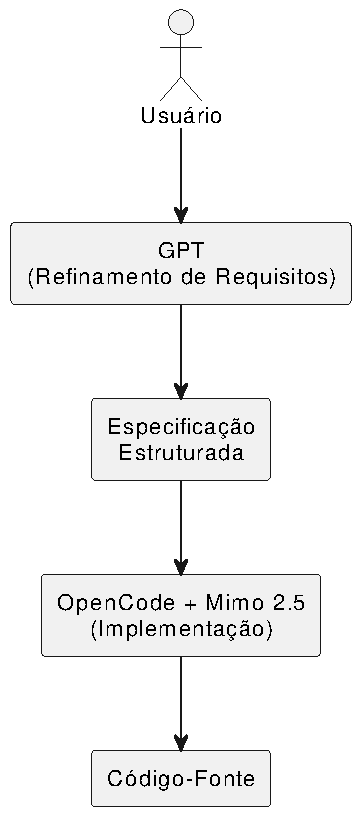
\includegraphics[width=1\linewidth,height=7.5cm,keepaspectratio]{imagens/fluxo-llm}
  \caption{Pipeline de desenvolvimento orientado por agentes para refinamento de requisitos e implementação de software}
  \Description{Fluxo de trabalho entre agentes}
\end{figure}

O agente refinador tem como objetivo transformar solicitações informais e com baixa aceitação pelas LLMs geradoras de código em estruturas mais detalhadas e específicas, auxiliando o desenvolvimento assistido por IA \cite{palermo_agentes_2026}. Para isso, uma descrição textual elaborada, identificando todos os objetivos de uma funcionalidade, regras de negócio, fluxos principais e critérios de aceite, deve ser passada para o modelo utilizado no refinamento \cite{ciudrowski2026explorando}. A LLM é capaz de identificar especificamente pontos de ambiguidade, omissão e inconsistências, aumentando a precisão dos requisitos refinados \cite{palermo_agentes_2026}.

Todos os textos devolvidos pelo modelo de refinação devem ser validados e interpretados para garantir o entendimento completo da funcionalidade, evitando que ela seja desenvolvida de forma incompleta ou incorreta \cite{tolio_llms_2026}. Um ponto de destaque é a importância de existir um profissional técnico por trás da criação desse texto inicial, para conduzir o refinamento orientando as bibliotecas usadas, as validações necessárias e outros pontos que podem impactar o desenvolvimento e a segurança do projeto \cite{ciudrowski2026explorando, palermo_agentes_2026}.

Nesse caso empírico, a escolha pela utilização do GPT se deu pela sua alta capacidade criativa e de escrita, se mostrando extremamente habilidoso no estruturação dos prompts \cite{minaee_large_2024}. Entretanto, entende-se que qualquer agente capaz de escrever prompts com qualidade pode ser usado nessa etapa de desenvolvimento.

Após o refinamento dos requisitos e especificações de implementação, o prompt gerado deve ser utilizado como entrada para o agente de desenvolvimento, utilizando o modo \textit{thinking} para que ocorra o pensamento e a criação do fluxo das tarefas refinadas pela outra LLM. A partir desse momento, o agente poderá efetuar questionamentos ao desenvolvedor, e esses devem ser analisados e respondidos conforme a necessidade do projeto \cite{minaee_large_2024}.

Todos os retornos de código devem ser analisados e verificados por um desenvolvedor com capacidade crítica de entender se o que foi feito possui manutenibilidade, confiabilidade e segurança \cite{ciudrowski2026explorando, palermo_agentes_2026}. As implementações devem seguir o padrão no qual seriam feitas pelo próprio desenvolvedor; com isso, ele deve ter total domínio da linguagem de programação utilizada para compreender a estrutura criada.

Um ponto de destaque é a importância de um arquivo com instruções para o agente se tornar mais técnico e específico no projeto, podendo ser um \textit{AGENTS.md} na raiz, especificando toda a arquitetura do projeto para que ele siga os padrões pré-definidos. O guia de arquitetura, funcionalidades, cores e skills utilizadas dentro desse arquivo funcionará como um manual de instruções para ele se basear e entender como deve estruturar as funcionalidades. Contudo, esse manual deve ser novamente refinado com um modelo de inteligência artificial generativo para deixá-lo descritivo e claro.

Dentro do projeto do editor em \LaTeX{}, foi proposta a utilização da ferramenta open-source OpenCode com o Mimo 2.5, por conta do seu baixo consumo de tokens e da capacidade de pensamento avançado disponível como opção antes da execução do desenvolvimento. Entretanto, é possível se utilizar de outras ferramentas e modelos para essa técnica, tendo em vista a necessidade de um desenvolvedor experiente e com conhecimento na área para tomar a decisão de qual utilizar no projeto.

Para avaliar a aplicabilidade da metodologia proposta, foi desenvolvida uma ferramenta de edição de textos acadêmicos. A ferramenta tem como objetivo auxiliar o processo de escrita, organização e revisão de documentos, integrando recursos tradicionais de edição com funcionalidades baseadas em inteligência artificial. As principais funcionalidades implementadas foram:

\begin{itemize}
    \item Criação, importação e clonagem de projetos a partir de repositórios Git;

    \item Listagem e gerenciamento dos projetos criados pelo usuário;

    \item Interface gráfica para edição de arquivos \texttt{.tex}, contendo recursos de leitura e manipulação do código-fonte;

    \item Criação, edição e organização de subpastas e arquivos dentro do projeto;

    \item Importação e gerenciamento de imagens utilizadas na composição dos documentos;

    \item Reorganização de arquivos e diretórios por meio de operações de arrastar e soltar (\textit{drag and drop});

    \item Visualização do PDF compilado diretamente na aplicação;

    \item Navegação por seções do documento, permitindo acesso rápido a capítulos e subseções por meio de âncoras;

    \item Download do documento PDF gerado;

    \item Inicialização de repositórios Git nos projetos e execução de comandos básicos de versionamento (em fase de aprimoramento para correção de inconsistências);

    \item Apresentação de mensagens de erro detalhadas durante o processo de compilação, facilitando a identificação e resolução de problemas;

    \item Integração com modelos de inteligência artificial para auxílio na revisão textual, incluindo correção ortográfica, análise de concordância verbal, melhoria de sentenças e identificação de repetição excessiva de termos. Foram utilizados modelos locais baseados em Llama e modelos disponibilizados pela plataforma Groq, permitindo que o usuário selecione o provedor desejado por meio de variáveis de ambiente;

    \item Desenvolvimento da documentação técnica do projeto utilizando a ferramenta MkDocs;

    \item Implementação de pipeline de integração e entrega contínua (CI/CD) para geração e publicação automática da documentação via GitHub Pages após alterações no repositório principal.
\end{itemize}

Como trabalhos futuros e itens presentes no backlog de desenvolvimento, destacam-se:

\begin{itemize}
    \item Implementação de uma análise completa do projeto utilizando inteligência artificial para identificar e sugerir correções ortográficas e gramaticais em todos os arquivos do documento, sem depender do arquivo atualmente aberto pelo usuário;

    \item Utilização de inteligência artificial para avaliar a aderência do conteúdo desenvolvido aos requisitos definidos pela banca avaliadora, identificando possíveis lacunas ou melhorias necessárias;

    \item Desenvolvimento de um recurso de assistência ao usuário para esclarecer dúvidas relacionadas à utilização de recursos \LaTeX, incluindo auxílio na aplicação de comandos de formatação textual, como negrito, itálico e outros elementos de estruturação do documento.
\end{itemize}

A Figura~\ref{fig:layout-sistema} apresenta o layout por dentro da ferramenta desenvolvida para apoiar a elaboração de textos acadêmicos em \LaTeX. A aplicação foi projetada para integrar, em um único ambiente, recursos como organização de documentos e assistência baseada em inteligência artificial.

Na interface, é possível observar a estrutura de arquivos do projeto, permitindo a navegação entre seções, imagens, referências bibliográficas e demais artefatos que compõem o documento. Foi utilizado o modelo padrão da conferência para exemplificar como seria um texto produzido por ele, além de ser testado de forma prática na construção desse artigo. 

A área central é destinada à edição do conteúdo em \LaTeX, enquanto o painel lateral exibe a visualização do PDF gerado em tempo real, possibilitando ao usuário acompanhar imediatamente os resultados das alterações realizadas.

Além das funcionalidades tradicionais de edição, a ferramenta incorpora recursos voltados a assistentes de IA para apoiar na escrita, refinamento de conhecimento e, em versões futuras, auxílio na utilização de comandos \LaTeX. Integrações com plataformas como GitHub também podem ser observadas na imagem, facilitando o gerenciamento e versionamento do projeto, facilitando a escrita em conjunto. Também é possível visualizar a navegação por sumário e exportação do documento em formato PDF, concentrando em uma única plataforma os principais recursos necessários para a produção de trabalhos acadêmicos.

A solução foi desenvolvida seguindo uma arquitetura de monolito modular, utilizando React no frontend e Express no backend. Para simplificar o processo de configuração do ambiente, diminuindo a dificuldade inicial em sua utilização, a infraestrutura é disponibilizada por meio de contêineres Docker, eliminando a necessidade de instalação manual de dependências e bibliotecas por parte dos usuários. Dessa forma, a ferramenta reduz o esforço inicial de configuração e permite que pesquisadores e estudantes concentrem suas atividades na produção do conteúdo acadêmico.

\begin{figure}[htbp]
  \centering
  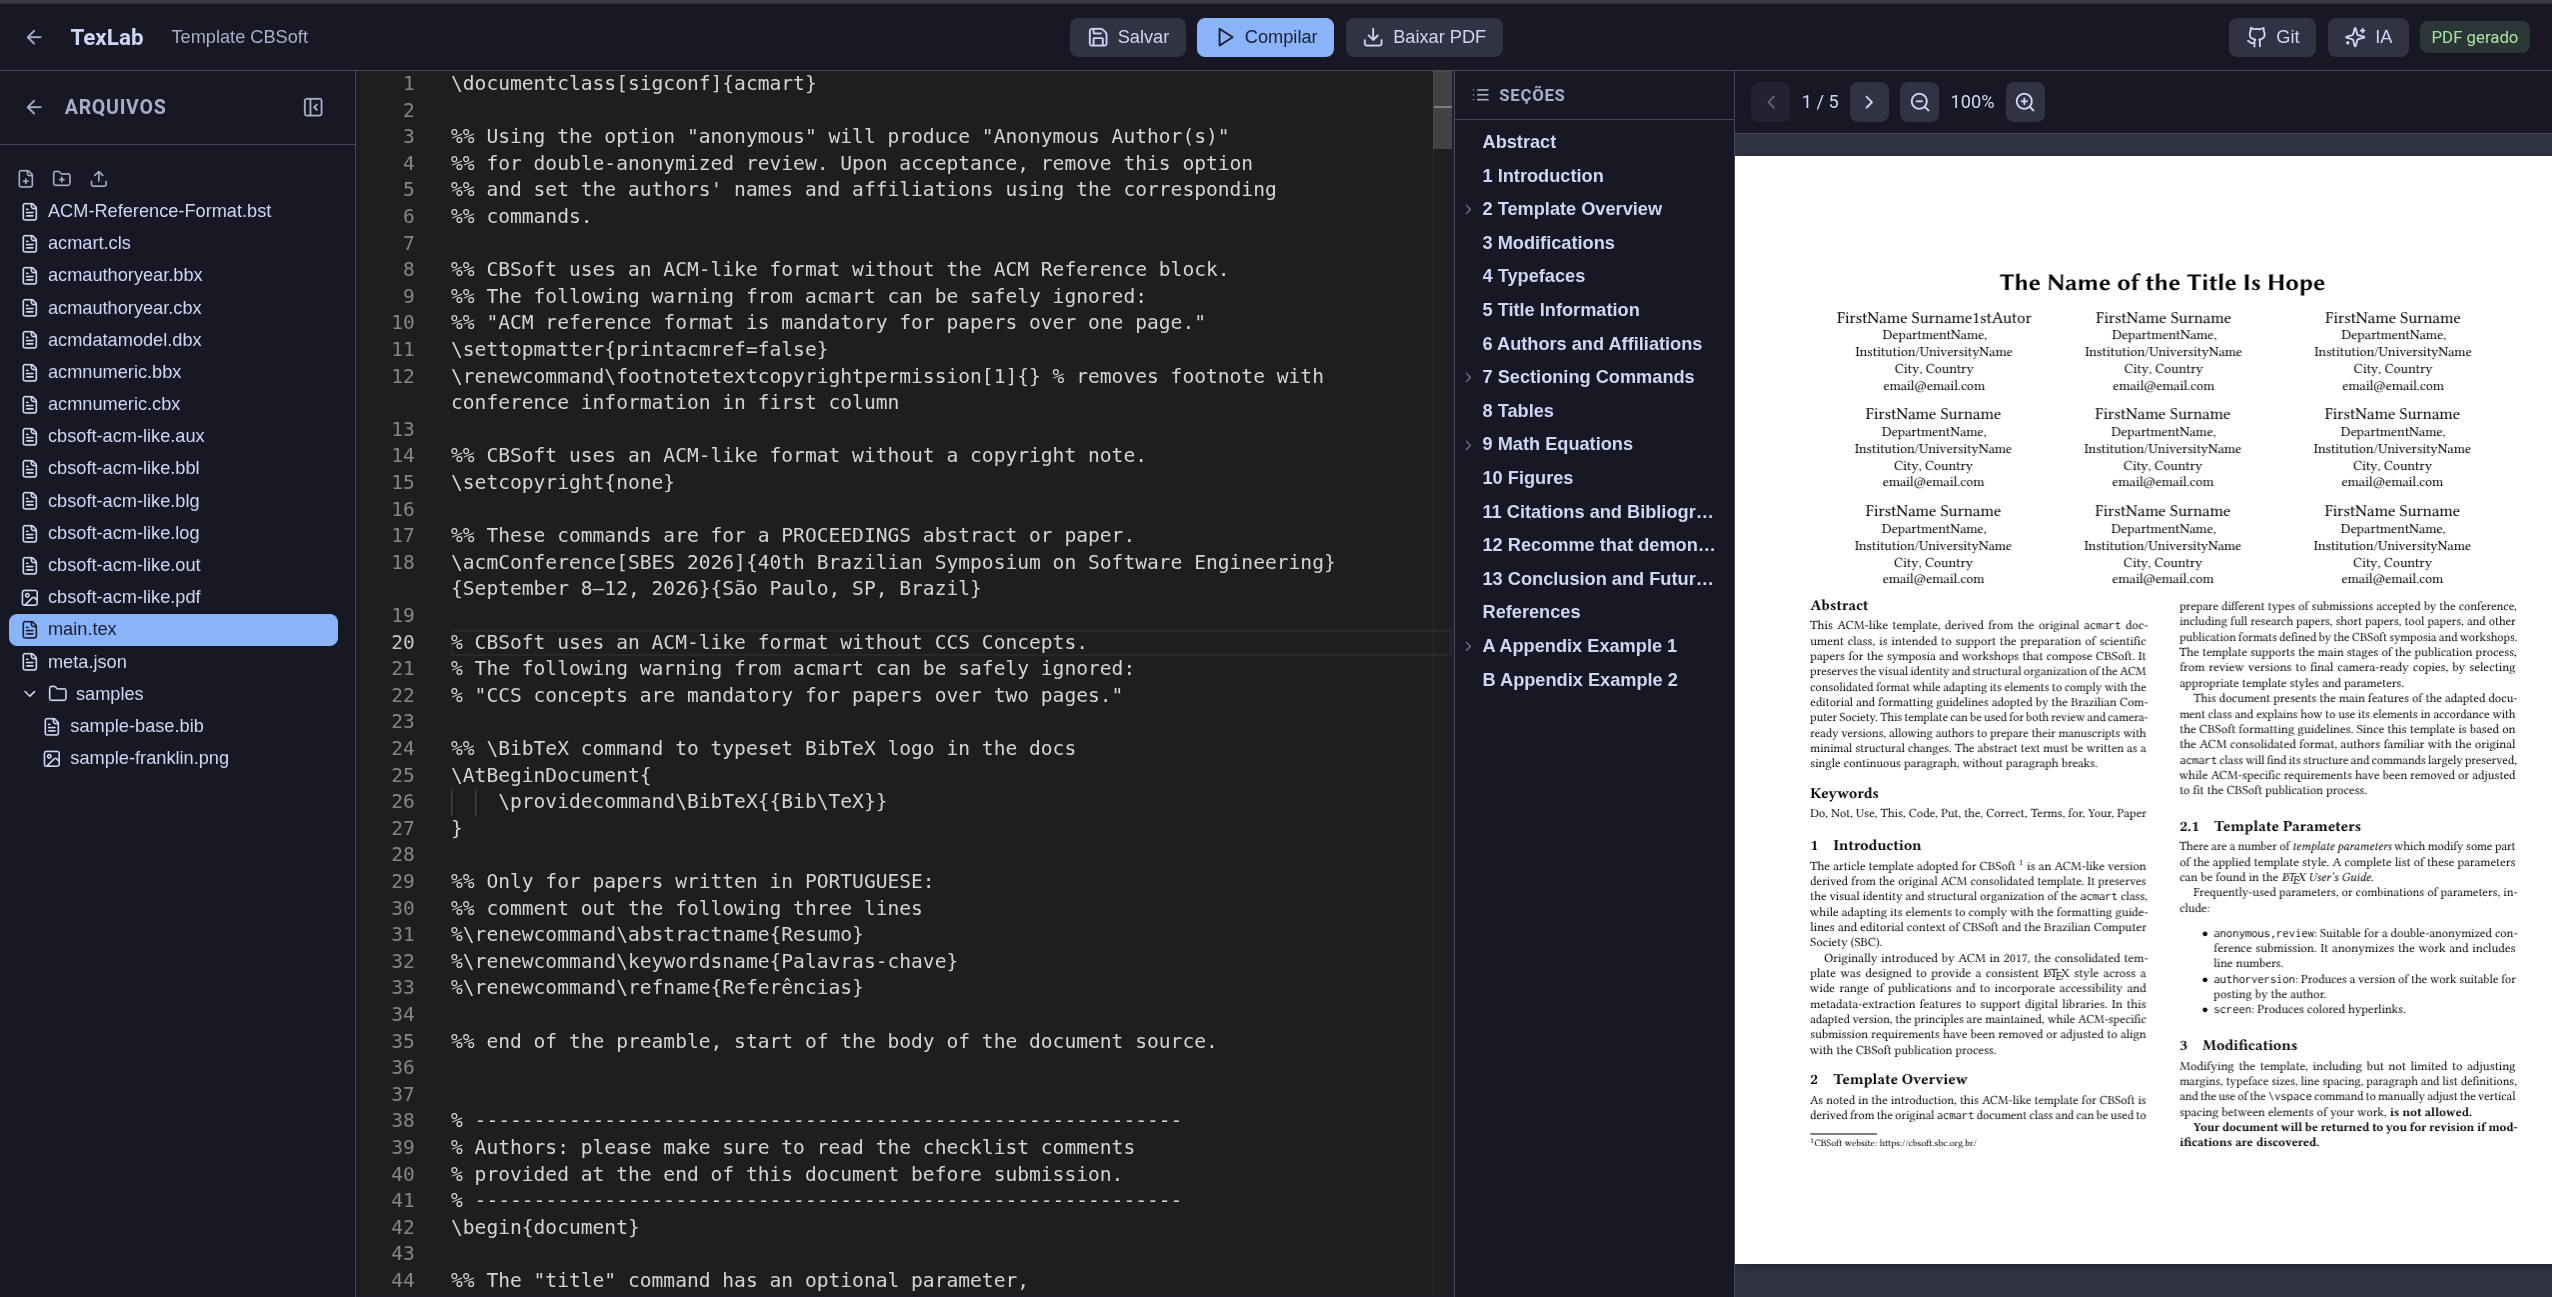
\includegraphics[width=\linewidth,keepaspectratio]{imagens/layout-texlab}
  \caption{Layout do sistema de edição de textos em \LaTeX.}
  \label{fig:layout-sistema}
  \Description{Layout do sistema}
\end{figure}

Durante o processo de desenvolvimento da ferramenta, foi observado que a utilização de uma LLM para realização do refinamento e criação do prompt contribuiu de forma positiva com os resultados. Ela auxiliou na robustez do prompt, consolidando a ideia, adicionando regras de negócio e requisitos não funcionais. Com isso, diminuiu a ambiguidade, inconsistências e melhorou a comunicação com o agente de desenvolvimento.

Funcionalidades simples puderam ser implementadas com um único prompt ou com poucas interações adicionais. Enquanto isso, funcionalidades mais complexas demandaram ciclos extras de desenvolvimento assistido pelo agente, sendo necessário testar a aplicação e entender onde não estava funcionando para explicar para o agente refinar um texto de melhoria.

A análise feita demonstrou a importância de um profissional técnico por trás para manusear a ferramenta durante o processo, conduzindo o modelo a produzir código com alta qualidade. Dessa forma, a metodologia não substitui o papel do desenvolvedor, mas busca ampliar sua produtividade por meio da automação de atividades de especificação e implementação.

Por fim, observou-se que a disponibilização de documentos de contexto, como o arquivo AGENTS.md contendo informações sobre arquitetura, convenções, padrões de layout e tecnologias utilizadas, contribuiu para aumentar a aderência das implementações aos padrões previamente definidos para o projeto.

\section{Citations and Bibliographies}

The use of \BibTeX\ for the preparation and formatting of one's references is strongly recommended. Authors' names should be complete. Use full first names (``Donald E. Knuth'') instead of initials (``D. E. Knuth''), and the identifying features of a reference must be included: title, year, volume, number, pages, article DOI, etc.

The bibliography is included in your source document with these two
commands, placed just before the \verb|\end{document}| command:
\begin{verbatim}
  \bibliographystyle{ACM-Reference-Format}
  \bibliography{bibfile}
\end{verbatim}

\verb|bibfile| is the \BibTeX\ filename without the \verb|.bib| suffix.

Citations and references are numbered by default. Some examples:
\begin{itemize}
\item A paginated journal article \cite{Abril07}
\item An enumerated journal article \cite{Cohen07}
\item A reference to an entire issue \cite{JCohen96}
\item A monograph (whole book) \cite{Kosiur01}
\item A monograph/whole book in a series \cite{Harel79}
\item A divisible book such as an anthology or compilation \cite{Editor00}
\item A divisible book (series not included since no volume number is given) \cite{Editor00a}
\item A chapter in a divisible book \cite{Spector90}
\item A chapter in a divisible book in a series \cite{Douglass98}
\item A multi-volume work as a book \cite{Knuth97}
\item Paginated proceedings articles \cite{Andler79, Hagerup1993}
\item A proceedings article with all possible elements \cite{Smith10}
\item An enumerated proceedings article \cite{VanGundy07}
\item An informally published work \cite{Harel78}
\item Preprints \cite{Bornmann2019, AnzarootPBM14}
\item A doctoral dissertation \cite{Clarkson85}
\item A master's thesis \cite{anisi03}
\item Online documents / World Wide Web resources \cite{Thornburg01, Ablamowicz07, Poker06}
\item Video games (Case 1) \cite{Obama08}
\item Video games (Case 2) \cite{Novak03, Lee05}
\item A patent (Case 3) \cite{JoeScientist001}
\item Work accepted for publication \cite{rous08}
\item `YYYYb' test for prolific author \cite{SaeediMEJ10, SaeediJETC10}
\item Citations containing duplicate DOI and URLs (e.g., some SIAM articles) \cite{Kirschmer:2010:AEI:1958016.1958018}
\item Multi-volume works as books \cite{MR781536, MR781537}
\item A presentation \cite{Reiser2014}
\item An article under review \cite{Baggett2025}
\item Citations with DOIs \cite{2004:ITE:1009386.1010128, Kirschmer:2010:AEI:1958016.1958018}
\item Online citations \cite{TUGInstmem, Thornburg01, CTANacmart}
\item Artifacts \cite{R, UMassCitations}
\end{itemize}


\section{Recomme that demonstratependices}

If your work needs an appendix, add it before the \verb|\end{document}| command at the conclusion of your source document.

Start the appendix with the \verb|appendix| command:
\begin{verbatim}
  \appendix
\end{verbatim}

In the appendix, sections are lettered rather than numbered. This document has two appendices that demonstrate the section and subsection identification method.

\section{Conclusion and Future Work}
<text included by the authors>

\section*{Artifact Availability}
This section must be included immediately after the Conclusion and before the Acknowledgments section. It must not be numbered and must be titled exactly as \textbf{Artifact Availability}.

If the paper provides research artifacts (such as datasets, source code, scripts, models, or experimental packages), the authors must describe what is available, where it can be accessed, and under which license or usage conditions.

If no artifacts are available, this section must still be included, explicitly stating that no artifacts are provided.

For papers written in Portuguese, this section must be titled
\textbf{Disponibilidade de Artefatos}.

\section*{Acknowledgements}
<text included by the authors>

%% The next two lines define the bibliography style to be used, and
%% the bibliography file.
\bibliographystyle{ACM-Reference-Format}
\bibliography{samples/sample-base}

%% If your work has appendices, this is the place to put them
\appendix

\section{Appendix Example 1}

\subsection{Part One}
Lorem ipsum dolor sit amet, consectetur adipiscing elit. Morbi malesuada, quam in pulvinar varius, metus nunc fermentum urna, id sollicitudin purus odio sit amet enim. Aliquam ullamcorper eu ipsum vel mollis. Curabitur quis dictum nisl. Phasellus vel semper risus, et lacinia dolor. Integer ultricies commodo sem nec semper.

\subsection{Part Two}
Etiam commodo feugiat nisl pulvinar pellentesque. Etiam auctor sodales ligula, non varius nibh pulvinar semper. Suspendisse nec lectus non ipsum convallis congue hendrerit vitae sapien. Donec at laoreet eros. Vivamus non purus placerat, scelerisque diam eu, cursus ante. Etiam aliquam tortor auctor efficitur mattis.

\section{Appendix Example 2}
Nam id fermentum dui. Suspendisse sagittis tortor a nulla mollis, in pulvinar ex pretium. Sed interdum orci quis metus euismod, et sagittis enim maximus. Vestibulum gravida massa ut felis suscipit congue. Quisque mattis elit a risus ultrices commodo venenatis eget dui. Etiam sagittis eleifend elementum.

Nam interdum magna at lectus dignissim, ac dignissim lorem rhoncus. Maecenas eu arcu ac neque placerat aliquam. Nunc pulvinar massa et mattis lacinia.

\end{document}

% ============================================================
% CBSoft ACM-like Template – Author Checklist
% ============================================================
%
% 1. Remove CCS Concepts
%    - Remove the CCSXML block and \ccsdesc commands.
%
% 2. Remove ACM footer
%    Use the command \renewcommand\footnotetextcopyrightpermission[1]{}
%
% 3. Remove ACM Reference Format
%    Use the commands \setcopyright{none} and 
%    \settopmatter{printacmref=false}
%
% 4. Short title must not exceed column width
%    Use the command 
%    \renewcommand{\shorttitle}{The Name of the Title Is Hope}
%
% 5. Include authors' surnames in the page headers (even pages)
%    - The author names in the page header (at the top of the page)
%      must not exceed the column width
%    - This list must contain only the authors' surnames
%    - Suggestion: use "Surname et al." for more than two authors with the
%      command \renewcommand{\shortauthors}{Surname1stAuthor et al.}
%
% 6. Author format below title:
%    \author{FirstName Surname}
%    \affiliation{
%      \institution{Department, Institution}
%      \city{City}
%      \country{Country}}
%    \email{email@email.com}
%
% 7. Verify all author emails are included
%    - Check font consistency
%
% 8. All numbered section and subsection titles must follow the same
%    capitalization style: the first letter of each word in the title 
%    must be capitalized (Title Case).
%
% 9. Artifact Availability (check CFP)
%    - Not numbered -- use \section*{Artifact Availability}
%    - Placed after Conclusion and before Acknowledgments
%    - In Portuguese, use \section*{Disponibilidade de Artefatos}
%
% 10. Abstract
%     - Single paragraph
%     - Papers written in Portuguese must use "Resumo" instead of "Abstract"
%       with the command \renewcommand\abstractname{Resumo}
%
% 11. Keywords
%     - Comma-separated, first letter capitalized
%     - Papers written in Portuguese must use "Palavras-chave" instead of
%       "Keywords" with the command 
%       \renewcommand\keywordsname{Palavras-chave}
%
% 12. References
%     - Not numbered -- already enforced by the template
%     - Papers written in Portuguese must use "Referências" instead of
%       "References" with the command \renewcommand\refname{Referências}
%
% 13. Acknowledgements
%     - Optional section
%     - Not numbered -- use \section*{Acknowledgements}
%     - In Portuguese, use \section*{Agradecimentos}
%
% 14. Remove received/revised/accepted dates
%
% 15. Figure captions must appear below figures
%
% 16. Verify the symposium name in the page header
%    - Use English, even if the paper is written in Portuguese
%    - Select the correct event according to the track
%    - Use Arabic ordinal numbers, not Roman
%
%    SBES (Research, Education, IIER, Tools, Industry)
%    \acmConference[SBES 2026]{40th Brazilian Symposium on Software Engineering}{September 8--11, 2026}{São Paulo, SP, Brazil}
%
%    SBLP
%    \acmConference[SBLP 2026]{30th Brazilian Symposium on Programming Languages}{September 8--11, 2026}{São Paulo, SP, Brazil}
%
%    SBCARS
%    \acmConference[SBCARS 2026]{20th Brazilian Symposium on Software Components, Architectures, and Reuse}{September 8--11, 2026}{São Paulo, SP, Brazil}
%
%    SAST
%    \acmConference[SAST 2026]{11st Brazilian Symposium on Systematic and Automated Software Testing}{September 8--11, 2026}{São Paulo, SP, Brazil}
%
%    Workshops
%    \acmConference[Workshop Acronym 2026]{Workshop Full Name}{Workshop Date}{São Paulo, SP, Brazil}
%
%
% 17. Remove colored author names, citations, and links
%
% 18. Camera-ready only:
%     Do not use the "review" or "anonymous" modes in the 
%     \documentclass command
%
% 19. SBES Tools Track papers must include a demo video link at the end of
%     the abstract
%     Example:
%     \begin{abstract}
%     <abstract text> \newline
%     \textbf{Demo video:} <video link>
%     \end{abstract}
%
% 20. SBES Industry Track papers must not include author biographies
%
% ============================================================

\endinput


